\documentclass[12pt,a4paper]{article}
\usepackage[a4paper, margin=2cm]{geometry}
\usepackage{graphicx}
\usepackage[table]{xcolor}
\usepackage{subcaption}
\newcommand{\tr}{\mathrm{tr}}
\usepackage{hyperref}
\usepackage{authblk}
\usepackage[backend=biber, style=chem-acs]{biblatex}

\bibliography{article}
\addbibresource{article.bib}


\begin{document}
\title{Ionizations of Liquid Water from Charged-cell Periodic Subsystem DFT and Embedded Simulations}
\author[1]{Jessica Martinez}
\author[1]{Pablo Ramos}
\affil[1]{Department of Chemistry, Rutgers University, Newark, New Jersey}
\author[2]{Andre Gomes}
\affil[2]{Université de Lille, CNRS, UMR 8523 – PhLAM – Physique des Lasers, Atomes et Molécules, Lille, France}
\author[3]{Johannes Tölle}
\affil[3]{Theoretische Organische Chemie, OrganischChemisches Institut and Center for Multiscale Theory and Computation (CMTC), Westfälische Wilhelms-Universität Münster, Corrensstraße 40, 48149, Münster, Germany}
\author[1]{Michele Pavanello\thanks{\textit{Email: m.pavanello@rutgers.edu}}}
\date{}
\setcounter{Maxaffil}{0}
\renewcommand\Affilfont{\itshape\small}
\begin{titlepage}
  \maketitle
\end{titlepage}

\begin{abstract}
Modeling the ionization potential (IP) of liquid water is challenging because the bulk-like nature of the liquid imposes
the use of periodic boundary conditions (PBCs), which pose roadblocks when considering charge systems; In this work, we tackle
this challenge by employing subsystem DFT to split the extended system into a collection of finite
subsystems embedded by extended, infinite subsystem. This is achieved by an impurity
model ~\cite{tolle2019charged} where different Density Functional Theory (DFT) can be introduced 
to evaluate the water molecules’ energy. \\

The liquid’s electronic structure is expressed in subsystem contributions by invoking nonadditive density 
functionals whereby the total energy of the liquid is expressed as the sum of molecule-additive
and nonadditive contributions ~\cite{krishtal2015subsystem}. The inter-molecular interaction is
split into Coulumb interactions, and such nonadditive terms as the noninteracting
kinetic energy and the noninteracting exchange-correlation ~\cite{krishtal2015subsystem}. 
These contributions represent interactions related among others to exchange, van der Waals and
Pauli repulsion and are all bifunctional of the subsystem densities ~\cite{tolle2019charged}. \\

The final IP values reproduce the experimental values to within 0.5 eV and are determined averaging 
over multiple systems of 64 water molecules (or subsystems) considered in the corresponding simulation
cell, calculated by the energy difference of the neutral and the polarized system (Called SCF method) 
~\cite{bagus1965self,waskom2017mwaskom}.\\
\end{abstract}


\section{Introduction}

The high-accuracy calculations of ionization potentials (IPs) and electron affinities (EAs) of condensed-phase molecular systems as liquid water have 
represented a challenge for the last years in both experimental and computational fields
\cite{tolle2019charged,gaiduk2018electron,gaiduk2016photoelectron,seidel2016valence}. Thus, ionized states of the electrons take part in many
crucial processes in electrochemistry, photochemistry as well as peculiar states of matter like excess electrons solvated in liquid water
\cite{ambrosio2017electronic}. One of the most recent theoretical reports of IP value were determined through coupling path-integral molecular
dynamics with ab initio potential, and many-body perturbation theory (MBPT) at $G_{0}W_{0}$ level of theory by Gaiduk et al. \cite{gaiduk2018electron}.
Based on this study the Ionization Energy(IE) was determined to be 10.25 eV. In concordance Ziaei et al. 
through self-consistent GW approach with an implicit vertex correction based on the
projector augmented wave (PAW) method, which is the most accurate pseudo-potential \cite{dal2014pseudopotentials} (PPs available),
and combined with Bethe–Salpeter equation determined a close value of 10.26 eV \cite{ziaei2018probing}. In both studies, the value of IP 
corresponds to the valence band maximum (VBM) of the Electronic Density of States (EDOS), which were then corrected for reference to the vacuum level. \\

More recent work by Perry et al. \cite{perry2020ionization} resolved experimentally the ionization energy of liquid water in the presence of a tunable
bias voltage applied to liquid jet employing monochromatized high-harmonic light source. The above suggests values of the vertical and adiabatic
ionization energies of the $1b_1$ orbital band of bulk liquid water of 11.67 and 10.12 eV, respectively. Using 
self-consistent hybrid (sc-hybrid) functionals were predicted values of 11.15 \cite{pham2017electronic} and 11.24 \cite{gaiduk2018electron} 
eV for the vertical IP and 10.08 eV for the adiabatic IP \cite{pham2017electronic, gaiduk2018electron} ,
the later is determined by the linear extrapolation of the $1b_1$ peak of water to zero. 

Following the trend and now including the use of periodic boundary conditions (PBC) another method was introduced \cite{tolle2019charged}
to determine the ionization potentials (IPs) of liquid water. Based on the successful determination of a quantum-mechanical
model for charged species in PBC which is able to face the complications related to the long-range nature of the Coulomb Kernel
$ w(r,r^{'}) = \frac {1}{|r - r^{'}|}$, which decays to zero when two charges are far away in real space. Indeed, it was achieved using an impurity
model with two remarkable qualities: 1) The charged periodic system is replaced by a non-periodic one which is still truly
extended (ie., of infinite size) and 2) The potentials of the neutral and the charged system are pegged to a common reference. \\

The former requires an ad hoc mapping of the infinite system (periodic) onto finite number of finite subsystems (non-periodic subsystems) and an
extended (infinite) subsystem, using a formally exact density embedding method, subsystem DFT \cite{wesolowski2015frozen}. Meanwhile, achieving
the latter only requires finding a consistent choice for the $G = 0$ component of the Coulomb Kernel in a reciprocal space. 
The use of the reciprocal space is only chosen for avoiding the complication of dealing with convergent integrals \cite{martin2004electronic}
In addition, in PBC the physical Coulomb kernel is only the one represented in a reciprocal space $w(G) = \frac {4\pi}{|G|^2}$ where
$G \epsilon {\rm I\!R}^3$. Even though, when $G=0$ the Coulomb kernel becomes undefined the total charged density $\rho (G)$ is zero for $G = 0$
, which is not problematic.\\

Here we present an update of the current state-of-the-art of the liquid water IPs base on an impurity model using an exact density
embedding method, subsystem DFT. This may allow us to contribute to the discussion generated about the most accurate value for the IPs of bulk water
by using ab initio electronic structure \cite{ambrosio2017electronic, gaiduk2018electron} by GW approximations. We begin with a brief theoretical
framework description and followed with the description of the IPs of in principal on a 64 bulk liquid water system and afterward using the first
30 snapshots from Gaiduk et al. PI-MD simulations.

\section{Theoretical Background}

\subsection{Mapping a periodic system into a collection of non-periodic subsystems and one periodic subsystem}

To cast DFT in a subsystem fashion, we invoke nonadditive functionals in which each energy term of the supersystem is expressed as the sum of
additive and nonadditive contributions ~\cite{martyna1999reciprocal}. Therefore, when dealing with a finite subsystem with electron density
$\eta_I$, and an infinite or extended subsystem with electron density $\eta$ - $\eta_I$, the total density can be defined as the sum of the
finite subsystem and the extended subsystem, and the total energy is given by, \\

\begin{equation}
	E_{tot} = {E_[{\eta}_I]} + {E_[{\eta} - {\eta}_I]} + {E^{int}[{\eta}_I, {\eta} - {\eta}_I] } 
\end{equation}

The interaction energy can be broken down into the following contributions,

\begin{equation}
	E^{int} = E^{int}_H + V^{int}_eN + T^{nad}_s + E^{nad}_{xc} 
\end{equation}

The two Coulombic terms $E^{int}_H$ and $V^{int}_eN$ are the electron-electron and electro-nuclear interactions, respectively. And the
nonadditive terms $T^{nad}_s$ and $E^{nad}_{xc}$, represent the noninteracting kinetic energy of the system and the noninteracting
exchange-correlation functionals, respectively ~\cite{krishtal2015subsystem}. The two last terms represent interactions related among other to exchange, van der Waals and Pauli repulsion and are all bifunctional of the two subsystem densities. \\

\subsection{Coulomb interaction energy determination}

As the electron-nuclear interaction can be treated in an equivalent way that the Hartree terms of the interaction energy, with the definition of
the latter, we can map the complete theoretical background. The Hartree interaction energy then is defined between finite and infinite
electronic system by, \\

\begin{equation}
	E^{int}_H = \int_{{\rm I\!R}^3} dr \int_{\Omega} dr' \frac{1}{|r-r'|} [\eta(r)-\eta_{I}(r)]\eta_{I}(r') 
\end{equation}

The integral over $dr'$ takes place only over a finite volume $\Omega$, here represented by the simulation cell. Contrariwise, the integral in $dr$
is carried out over the entire space, due to the density $\eta -\eta_{I}$ is extended. \\

To describe the periodic potential interaction with a finite charge, first, we define the finite potential (define by an overbar) as being the potential which uses $\eta_{I}$ (the electron density of the finite subsystem), as, \\

\begin{equation}
	\bar{v} [\eta_I](r) = \int_{\Omega} dr' \frac{1}{|r-r'|} \eta_{I}(r')
\end{equation}

For equations $(3)$ and $(4)$ the integral over $dr'$ is carried out only over a finite volume $\Omega$ (typically the simualtion cell) because we expect $\eta_{I}(r)=0$ when $r \not\in \Omega$. \\

Therefore, computing the potential generated by the periodic system and using that in the computation of the interaction energy $E_{int}$,
which is defined as,

\begin{equation}
	E_{int} = \int_{\Omega} dr [v[\eta](n)-\bar{v}[\eta_{I}](r)]\eta_{I}(r)
\end{equation}

Where $v[\eta](n)$ is the full periodic potential. The potentials are evaluated separately, in which the finite potential is commonly solve in real 
space because $\eta_{I}$ is often the electron density of a finite system. \\

To compare total energies from periodic calculations the Coulomb kernel needs to be correctly referenced. In this work particularly, it is achieved 
imposing the $G=0$ value of the periodic Coulomb kernel to match the same limit of the Coulomb kernel of a reference system. Here we choose the
finite system to be the reference system. Thus, we referenced the periodic potential of the extended subsystem ($\eta -\eta_{I}$) to the corresponding
$G=0$ component in the the ionized and neutral systems. \\

\subsection{Embedding Scheme for the Nonionized System}

For the neutral system, the Coulomb interaction energy can be expressed as a potential that maps the interaction of an accurately infinitely extended
environment onto and isolated subsystem $I$, \\

\begin{equation}
	v^{I}_{emb} [\eta] (r) = v[\eta](r) - \bar{v} [\eta_I](r)
\end{equation}

Where $v[\eta](r)$ is the total Coulomb potential of the system and $\bar{v} [\eta_I](r)$ the potential of the isolated subsystem $I$. The latter was
evaluated using the Martyna-Tuckerman method whereby density $\eta_I$ is assumed to be isolated and not periodic \cite{martyna1999reciprocal}.
The embedding potential for the neutral subsystem can also be calculated directly from equation $3$. \\

\subsection{Impurity Model for the Ionized system}

To obtain the embedding potential of a charged subsystem, we consider the system to be composed of an ionized subsystem embedded in a nonionized
environment. To assemble the appropriate embedding potential, first was evaluated a screening potential, 
$v^{screen}[\eta_I](r) = v[\eta_I](r) - \bar{v} [\eta_I](r)$, understood as the electrostic potential of the periodically repeating water
molecules have on a single lattice site, achiving the removal of only one isolated subsystem. The later $\bar{v} [\eta_I](r)$ is evaluated by
Martyna-Tuckerman method\cite{martyna1999reciprocal}. The embedding potential depends on three densities: $\eta$ the total system,
$\eta_I$ the neutral subsystem, and $\eta^{'}_I$ the charged subsystem, and has the form, \\

\begin{equation}
	v^I_{emb,imp}[\eta, \eta^{'}_I, \eta_I](r) = v[\eta, \eta^{'}_I, \eta_I](r) - \bar{v}[\eta^{'}_I](r)
\end{equation}

with

\begin{equation}
	v[\eta, \eta^{'}_I, \eta_I](r) = v[\eta](r) + \Delta{v}^{screen}[\eta_I, \eta^{'}_I](r)
\end{equation}

where $\Delta{v}^{screen}[\eta_I, \eta^{'}_I](r) = {v}^{screen}[\eta_I](r) - {v}^{screen}[\eta^{'}_I](r)$, which replace the
electrostatic environment given by periodic images of the ionized subsystem having charged density $\rho^{'}_I$ with the neutral charged
density $\rho_I$ of the nonionized subsystem.

\section{Computational Section}

Embedding potentials for ionized and nonionized systems were obtained with embedded Quantum ESPRESSO (eQE) \cite{genova2017eqe}
employing ultrasoft pseudopotentials from PSL pseudopotential library \cite{corso2014comput}. PBE exchange-correlation functional 
\cite{perdew1996phys} was used to evaluate the additive and nonadditive contributions to the total energy, and revAPBEK
\cite{laricchia2011generalized} to the nonadditive Kinetic energy functional. Following previously benchmarking studies
\cite{genova2016avoiding, genova2017cooperation} a total of 40 Ry and 400 Ry were set as the energy cutoffs for the plane wave 
expansions of the molecular orbitals and the charge density, respectively.  \\

The ground state calculation of each subsystem with the corresponding neutral and polarized embedding potential was determined through ADF
\cite{te2001chemistry} software. We selected each water molecule to be one subsystem (i.e, 64 subsystems in total) according to the most beneficial
error cancelation, previously determined
\cite{genova2016avoiding, kevorkyants2013calculating, pavanello2011modelling, ramos2016critical, solovyeva2012spin},
between the nonadditive kinetic energy and the nonadditive exchange-correlation functionals employed. \\

To make use of the embedding potential (EP) for both neutral and charged systems (obtained by eQE) in the ADF ground-state
calculations, the atom centered grid function of eQE was used. The above is based on an interpolating function which 
splines the EP onto a custom grid, which provided the correct real-space representation due to the uses of atom centered
basis functions. The general integral has the form, \\

\begin{equation}
	v_{emb}^{\mu v} = \langle \chi_{\mu}|v_{emb}|\chi_{v}\rangle 
\end{equation}

This will generate a Gaussian cube file containing the splined embedding potential\cite{genova2017eqe}.

A comparison among Density Functional Theory (DFT), using GGA (PBE) \cite{perdew1996phys}, Hybrid (B3LYP) \cite{hertwig1997parameterization}, 
and Statistical average of orbital potentials(SOAP) model\cite{schipper2000molecular, gritsenko1999approximation}, 
Møller–Plesset perturbation theory (MP2) \cite{head1988mp2} and Hartree–Fock (HF) \cite{marshall1961unrestricted} level of theory was made, with the basis QZ4P. \\ 

The final IP values are calculated using an average for each of the 64 water molecules or subsystems considered in the simulation cell, 
for both the representative snapshot and the 25 first snapshots from Gaiduk et al. calculated by the energy difference of the neutral
and the polarized system (Called $\Delta$SCF method) \cite{bagus1965self,waskom2017mwaskom}.

\section{Results}

Using a random method a representative snapshot from an ab initio molecular dynamics (MD) based on subsystem DFT was selected base on a
previous study \cite{genova2016avoiding}. We used that single snapshot which consists of a total of 64 subsystems
(ie. 64 water molecules in a cubic box (a = 12.43 $\AA$) to compute the IPs reproducing the density of the liquid. \\

The IPs were calculated in two ways: Isolated, each subsystem was computed independently and treated using MT
assume isolated method \cite{martyna1999reciprocal}, all the molecular geometries were taken from the MD. Embedded: 
we employed the impurity model above described by equation $(7)$ and calculated the interaction energy following 
equation $(5)$. The coulomb kernel of the $\eta -\eta_{I}$ extended neutral system, was taken as a reference because of
their similarity between the neutral and ionized states, Figure S1. \\

We divided the succeeding analysis into two crucial parts. A complete comparison between previous eQE results \cite{tolle2019charged} for the
IPs of bulk water with ADF calculation using the same PBE functional. Followed by the description of IP results among the different 
DFT functionals, and their corresponding comparison with MP2. In addition, a short outline between HF and MP2 results.\\

\begin{table}[!ht]
\begin{center}
\setlength{\tabcolsep}{18pt}
  \caption{The average ionization potential in eV of liquid and gas-phase water in comparison to recent literature for both experimental and theoretical results. GW A, carried out with classical nuclei \cite{gaiduk2018electron}.GW B, uses quantum nucleia via a path integral dynamics \cite{gaiduk2018electron}. GW-PAW, uses implicit vertex correction based on projector augmented wave method\cite{ziaei2018probing}}
  \rowcolors{3}{gray!25}{white}
  \label{tab:table1}
  \begin{tabular}{ ccc }
  \hline
          Method &Gas-Phase& Liquid \\
  	\hline
          eQEcs&13.76&10.52\\
          eQEos&12.72&9.49\\
          MP2&13.18&9.9\\
          HF&10.98& 7.83\\
          PBE&12.80&9.61\\
          B3LYP&12.71&9.51\\
          SAOP&12.78&9.59\\
          GW A \cite{gaiduk2018electron} &- &10.55\\
          GW B\cite{gaiduk2018electron} &- &10.25\\
          GW-PAW\cite{ziaei2018probing} &- &10.2 \\
          exp A \cite{winter2004full} &- &9.9 \\
          exp B \cite{delahay1981chem} &- &10.06 \\
          exp \cite{nist2015nist} &12.62 &- \\
  	\hline
  	\end{tabular}
 \end{center}
\end{table}

The previous result for IPs of the 64 bulk water system was obtained through eQE software using PBE functional \cite{tolle2019charged}. 
Following the same theoretical framework (PBE) once we obtained the cube file for the splined embedding potentials, a Frozen Density 
Embedding (FDE) calculation was carried out with ADF for each subsystem. \\

As shown in Figure 1, the results for IPs of isolated water, (computed considering every single
molecule of the liquid to be isolated) evidenced that both histograms are peaked around the average
and only spreads by about 0.1 eV. If we compare isolated and bulk IPs histograms,
bulk IPs are much broader by about 2 eV. The above agree completely with the fact that the first
absorption band in the liquid, for the optical spectrum of water \cite{blase2016erratum,genova2017cooperation,hermann2008resolving,hahn2005optical},
peaks at higher energies in comparison to the gas-phase \cite{tolle2019charged}. Averages IPs for the bulk water are lower by ~2.2 and 3.3 eV
(calculated by eQE and ADF, respectively) than the IPs of the isolated system, which are in complete agreement
with experimental previously reported \cite{nist2015nist} gas-phase IPs. \\

In contrast to reported gas-phase IP values by Th{\"o}le et al.\cite{tolle2019charged} using eQE (Figure 1. Right) using Closed-Shell (CS)
we present a difference of about 1.0 eV, explained because the usage of open-shell of each ground-state calculation plays a crucial role in the determination of the  High occupied molecular orbital (HOMO) energies when a hole is added to the system. \\

\begin{figure}[!ht]
        \captionsetup[subfigure]{labelformat=empty}
        \centering
        \begin{subfigure}{0.4\linewidth}
                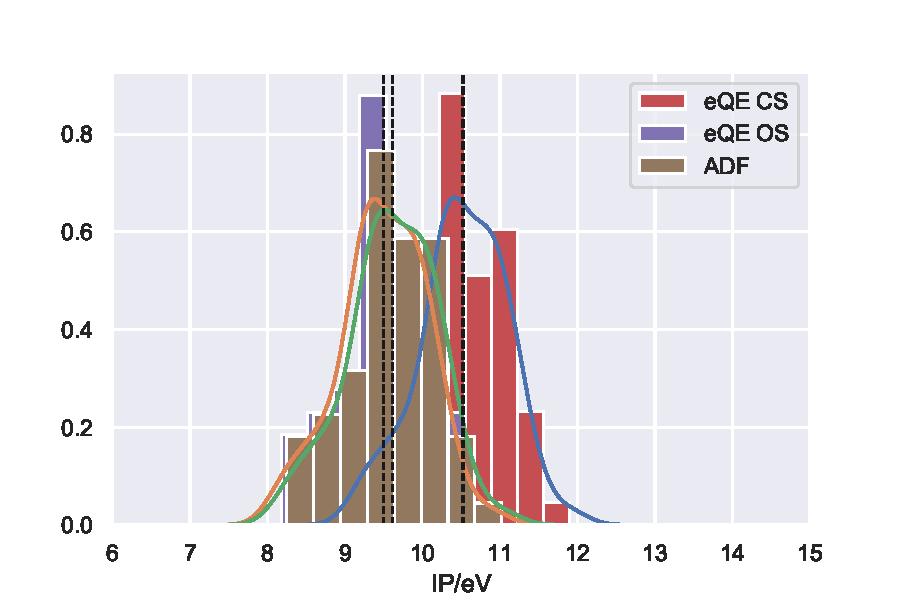
\includegraphics[width=\linewidth]{images/bulk-eqe-adf}
                \caption{Bulk Liquid Water}
        \end{subfigure}
        \begin{subfigure}{0.4\linewidth}
                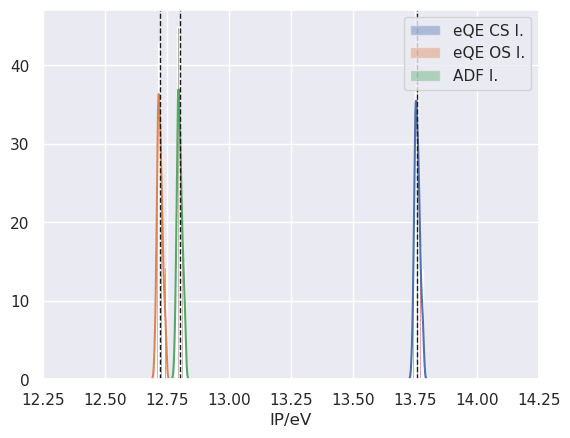
\includegraphics[width=\linewidth]{images/Iso-eqe-adf}
                \caption{Isolated}
        \end{subfigure}
        \caption{Comparison of the distribution of IPs of bulk liquid water between ADF\cite{te2001chemistry} and eQE \cite{genova2017eqe}. The area subtended by the lines sums up to 64 (ie, the number of subsystems). Left: Embedded water molecules in the bulk. Right: Isolated water molecules. Dot lines represent the average IP. The lines fitting the underlying distributions are obtained from a kernel density estimation using Seaborn's Gaussian envelopes\cite{waskom2017c}}
\end{figure}

Furthermore, there is an underestimation of the computed IP for bulk water through ADF in comparison with eQE CS calculations of 0.91
eV. We can argue the above recalling that eQE uses pseudopotential approximation that set the ion core electrons to 
be 'frozen' assuming they are not by definition perturbed by physical rearrangements of the system
\cite{srivastava1987theory}, while ADF treats core orbitals from high-level all-electron atomic calculations
to be frozen (but intact), calculating the atomic wavefunctions considering the complete system (i.e. all the
electrons)\cite{te2001chemistry}. However, once one calculates the charged subsystem under an open-shell setup
is possible to almost superimpose ADF and eQE IP with a difference of ~0.11eV. Being remarkable the use of 
Open-Shell configuration under the Frozen Density Embedding procedure.  \\

The IPs average between PBE and B3LYP functionals of the bulk liquid water present a difference of ~0.1 eV,
Figure 2 and Table 1. The first as a generalized gradient approximation (GGA) functional for the exchange-correlation
(XC) which description of the density $\rho$ depends not only at a certain point, but also the gradient of
$\rho$ at the point, could be calling 'non-local'\cite{perdew1996phys}. While the latter belongs
to the hybrid approximation which defines the exchange-correlation as the inclusion of some Hartree-Fock
exchange (HF) mixed with GGA exchange and correlation, plus some empirical parameters, making it certainly 
non-local \cite{hertwig1997parameterization}.  This leads to conclude that the non-locality framework plays a 
crucial role when an embedding potential is used. \\

SAOP (Statistical average of orbital potentials) model is an asymptotical correction of the XC designed to model
the Kohn-Sham (KS) potential with its Coulombic asymptotics for the occupied orbitals
\cite{chong2002interpretation, van2014physical},
If we compare B3LYP with the latter in the calculation of IPs liquid water there is a difference of 0.075 eV, 
however, in comparison with the experimental values both underestimate the IPs by ~0.4 eV.  \\

Analyzing this first section, the above XC functionals, with the second-order M$\o{}$ller-Plasset (MP2), 
which is an effective Hartree-Fock ground state energy correction for the electron correlation effects
\cite{del2012second}, we can argue that the difference of ~0.4 eV displayed in Figure 2 and Table 1, among MP2 and 
DFT methods used here is due to the not exact XC treatment of DFT calculations. \\

\begin{figure}[!ht]
        \captionsetup[subfigure]{labelformat=empty}
        \centering
        \begin{subfigure}{0.4\linewidth}
                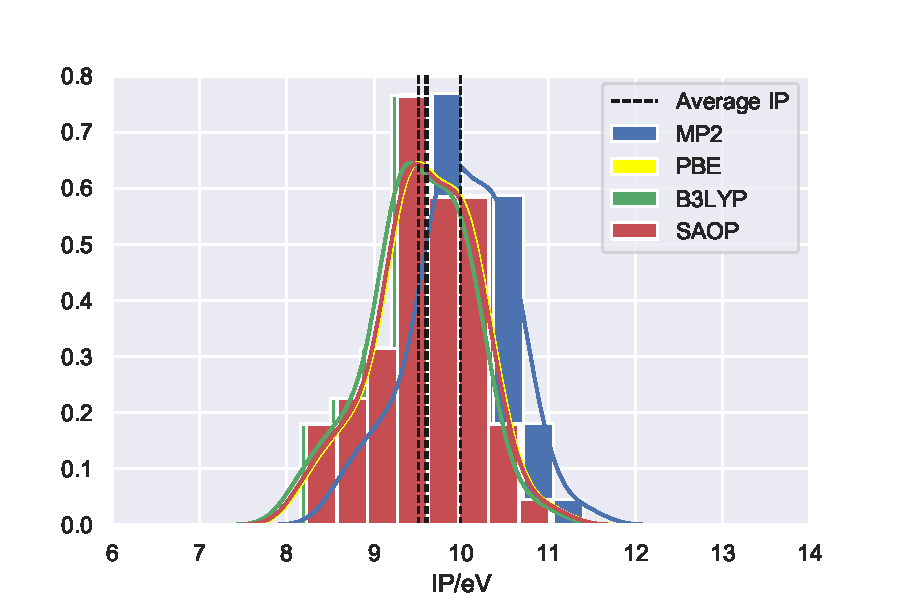
\includegraphics[width=\linewidth]{images/bulkmp2dft}
                \caption{Bulk Liquid Water}
        \end{subfigure}
        \begin{subfigure}{0.4\linewidth}
                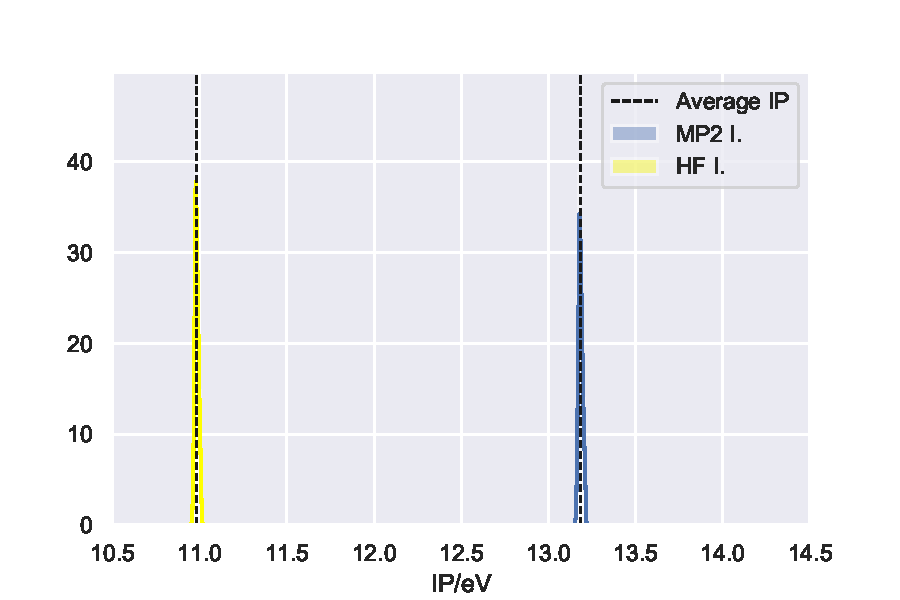
\includegraphics[width=\linewidth]{images/isomp2dft}
                \caption{Isolated}
        \end{subfigure}
        \caption{Distribution of IPs of bulk liquid water using MP2 and DFT methods through ADF \cite{te2001chemistry}. The area subtended by the lines sums up to 64 (ie, the number of subsystems). Left: Embedded water molecules in the bulk. Right: Isolated water molecules. Dot lines represent the average IP. The lines fitting the underlying distributions are obtained from a kernel density estimation using Seaborn's Gaussian envelopes\cite{waskom2017c}}
\end{figure}

Even though MP2 is one of the oldest and the simplest wave function-based approaches to electron correlation energy
it is still an eminent method 
of quantum chemistry in which its energy contribution consists of double excitations \cite{fink2016does}. 
Above provides a systematic way to
improve the description of the dynamic correlation energy, and in comparison with HF\cite{marshall1961unrestricted} 
wich entirely neglects these 
effects let us figure out that the dynamic correlation plays an important role in the establishment of IPs values.
Particularly, in Figure 4 and
Table 1, we can observed that HF underestimates the IPs with a difference of ~2.2 eV between HF and MP2,
which remarks again the importance of
include dynamic correlation in the liquid IP estimation. \\

\begin{figure}[!ht]
        \captionsetup[subfigure]{labelformat=empty}
        \centering
        \begin{subfigure}{0.4\linewidth}
                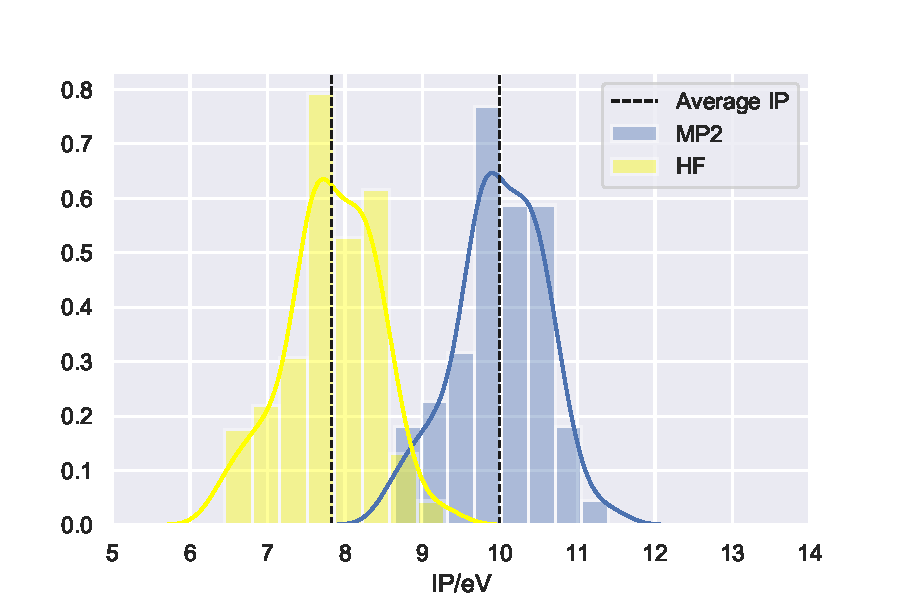
\includegraphics[width=\linewidth]{images/bulkhfmp2}
                \caption{Bulk Liquid Water}
        \end{subfigure}
        \begin{subfigure}{0.4\linewidth}
                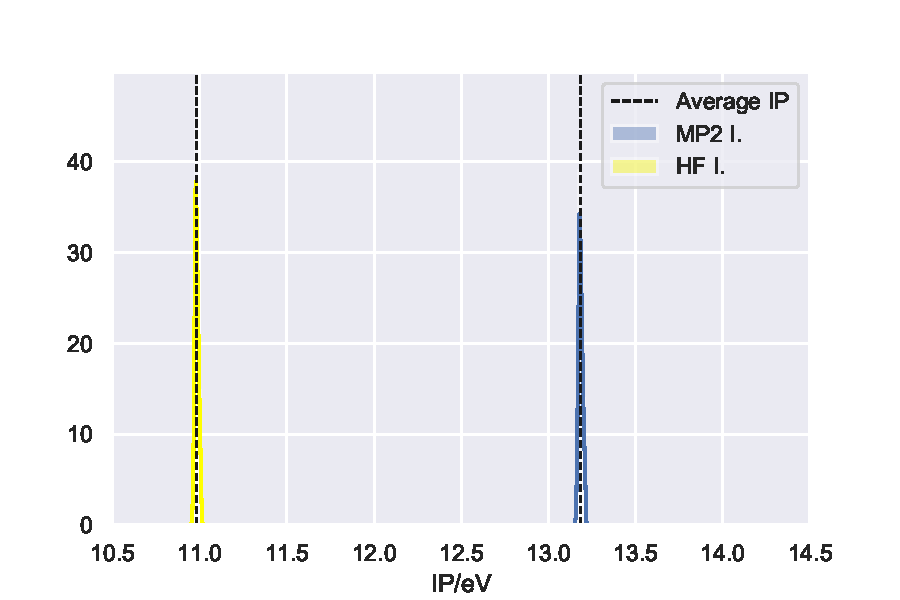
\includegraphics[width=\linewidth]{images/isomp2dft}
                \caption{Isolated}
        \end{subfigure}
        \caption{Distribution of IPs of bulk liquid water using MP2 and HF methods through ADF \cite{te2001chemistry}. The area subtended by the lines sums up to 64 (ie, the number of subsystems). Left: Embedded water molecules in the bulk. Right: Isolated water molecules. Dot lines represent the average IP. The lines fitting the underlying distributions are obtained from a kernel density estimation using Seaborn's Gaussian envelopes\cite{waskom2017c}}
\end{figure}

An extra term (Equation 9) was taking into account to add the Coulomb contribution of the interacting nuclei. Each subsystem was evaluated
separately, \\

\begin{equation}
        E_{int,nuc}^{0/+}=v_{emb}^{0/+}(R_{H_1}) Z_{H_1} + v_{emb}^{0/+}(R_{H_2}) Z_{H_2} + v_{emb}^{0/+}(R_{O}) Z_{O}
\end{equation}

Therefore, the contribution to the IP from the interaction with the nuclei to the IP is expressed as, \\

\begin{equation}
        \Delta IP = E_{int,nuc}^{+} - E_{int,nuc}^{0}
\end{equation}

This contribution is added to the preoviously determined "Electronic" IP for each subsystem. \\

\begin{equation}
IP_\alpha = IP^{electronic}_\alpha + \Delta IP_\alpha
\end{equation}

A brief comparison between the $1b_{1}$ peak of the optical spectrum of water among the non-$E_{int,nuc}^{0/+}$ contribution and including it
was made. This new term added leads the ionization potential increases of ~0.65 eV result which leads to a closer value to
the previously self-consistent GW approach, through PBE functional (Figure 7) and a overstimaion of ~0.4 eV using PBE. \\

\begin{figure}[!ht]
        \captionsetup[subfigure]{labelformat=empty}
        \centering
        \begin{subfigure}{0.4\linewidth}
		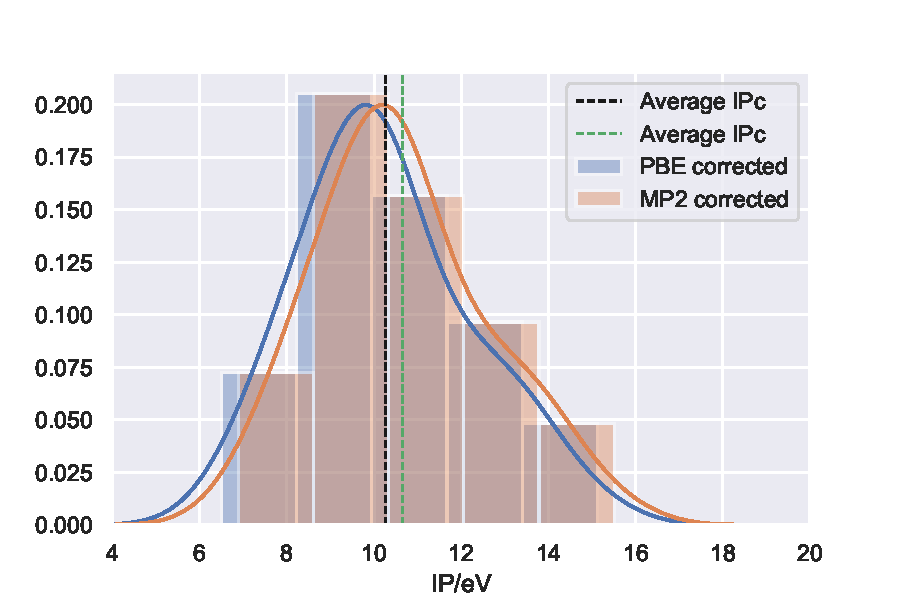
\includegraphics[width=\linewidth]{images/Corrected}
		\caption{Adding $E_{int,nuc}^{0/+}$ }
        \end{subfigure}
        \begin{subfigure}{0.4\linewidth}
                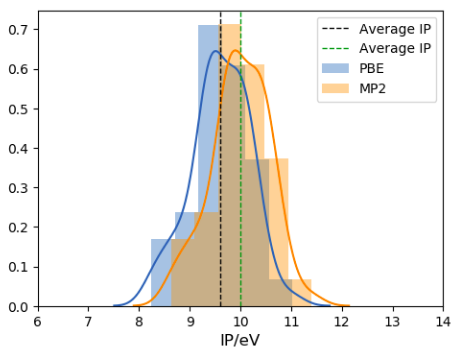
\includegraphics[width=\linewidth]{images/Without-Correction}
                \caption{Without $E_{int,nuc}^{0/+}$ }
        \end{subfigure}
        \caption{Distribution of IPs of bulk liquid water using MP2 and PBE method through ADF \cite{te2001chemistry} adding the extra term ($E_{int,nuc}^{0/+}$). The area subtended by the lines sums up to 69 (ie, the number of subsystems). Dot lines represent the linearly extrapolating from the ($1b_{1}$) peak. The lines fitting the underlying distributions are obtained from a kernel density estimation using Seaborn's Gaussian envelopes\cite{waskom2017c}}
\end{figure}

Last but not least we computed IPs of the first 25 snapshots of the complete trajectory of 64 water system using path-integral (PI) molecular
dynamics (MD) simulations from Gaiduk et al. \cite{gaiduk2018electron} (Figure 8) under the MP2 level of theory.
A total average IP of 9.96 eV among all the snapshots was obtained as a consequence of values between 9.81 and 10.03 eV
for the individual snapshots. If one compares those results with the most recent experimental adiabatic IP reported 
\cite{perry2020ionization} there is an underestimation of ~0.16 eV. 
However, following values of 9.9 \cite{winter2004full}and 10.06 eV \cite{kurahashi2014photoelectron} using photoelectron spectroscopy
our results are in completed agreetment.

\begin{figure}[!ht]
        \captionsetup[subfigure]{labelformat=empty}
        \centering
        \begin{subfigure}{0.4\linewidth}
                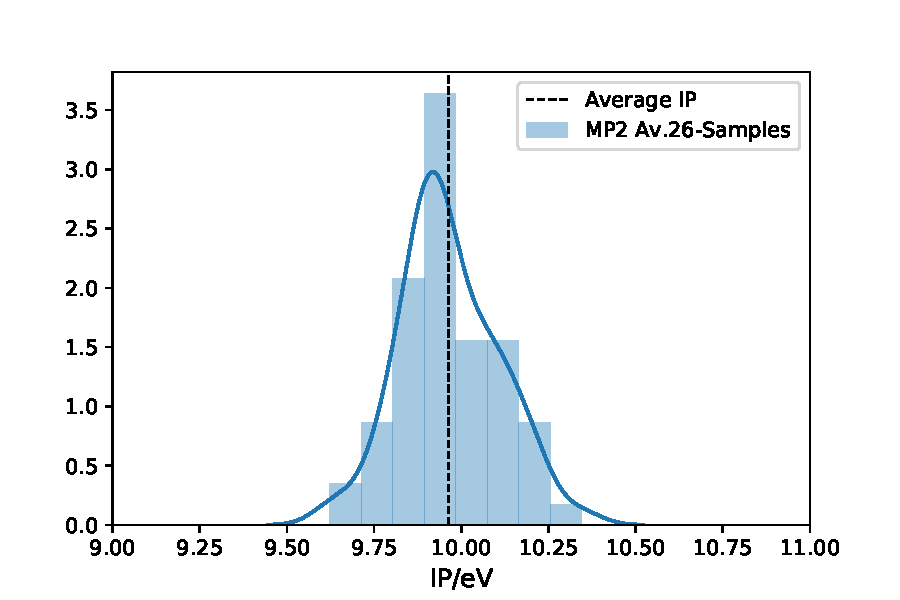
\includegraphics[width=\linewidth]{images/average30}
                \caption{Average}
        \end{subfigure}
        \begin{subfigure}{0.4\linewidth}
                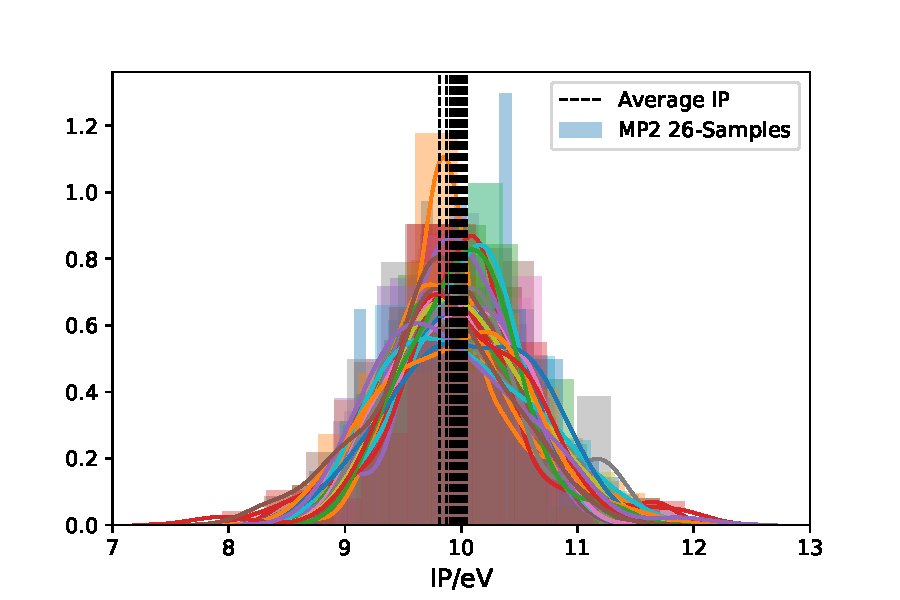
\includegraphics[width=\linewidth]{images/total30}
                \caption{Individual superporsition}
        \end{subfigure}
	\caption{Distribution of IPs of bulk liquid water using MP2 method through ADF \cite{te2001chemistry} for the first 25 snapshots of the PIMD from Gaiduk et al. The area subtended by the lines sums up to 64 (ie, the number of subsystems). Dot lines represent the linearly extrapolating from the ($1b_{1}$) peak. The lines fitting the underlying distributions are obtained from a kernel density estimation using Seaborn's Gaussian envelopes\cite{waskom2017c}.}
\end{figure}

\section{Conclusion}

Taking advantage of the density embedding depiction of the electronic structure of a system under periodic boundary conditions, we were able to 
compute through an impurity model that incorporates charged and neutral finite subsystems within an extended(infinity) surrounding subsystem, 
the IPs of bulk liquid water. So far, the best average value is 10.25 eV using the PBE level of theory adding the interaction correction to the 
nuclei which is in complete agreement with liquid experimental reported values (10.12 eV) and GW recent simulations (10.2-10.55eV). 
Future applications of the method will be aimed at the implementation of the embedding potential into the calculation of ionization potential
and electron affinities a higher level of theory. \\

\nocite{*}

\printbibliography

\section{Acknowledgments}


\end{document}
